\documentclass{article}

\usepackage[letterpaper,portrait,margin=1in]{geometry}

\usepackage{amsmath, amsfonts, amsthm, amssymb}
\usepackage{graphicx, float}
\usepackage{mathtools}
\usepackage{siunitx}
\usepackage{titlesec}
\usepackage{interval}
\usepackage{titling}
\usepackage{multicol}
\usepackage{siunitx}
\usepackage{vwcol}

\intervalconfig {
	soft open fences
}

\usepackage{tikz}
\usetikzlibrary{positioning}
\usetikzlibrary{angles,quotes}

\newtheorem*{theorem*}{Theorem}
\newcommand{\alignedintertext}[1]{%
	\noalign{%
		\vskip\belowdisplayshortskip
		\vtop{\hsize=\linewidth#1\par
		\expandafter}%
		\expandafter\prevdepth\the\prevdepth
	}%
}

%opening
\title{Problem Set \#33, Part 3}
\author{Jayden Li}
\date{December 11, 2023}

\begin{document}

\newgeometry{top=0.4in,bottom=1in,right=1in,left=1in}

\linespread{1.25}
\fontsize{12pt}{12pt}\selectfont

\maketitle

\section*{Problem 6}
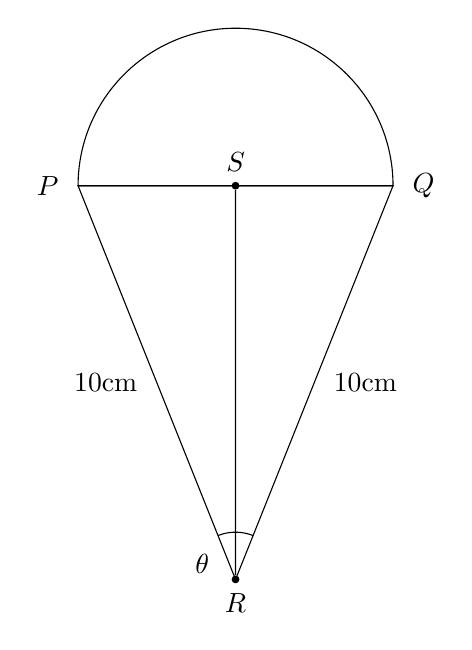
\begin{tikzpicture}	[
	baseline=(current bounding box.north),
	ang/.style={draw, angle eccentricity=1.5,angle radius=0.6cm}
]	
	\draw
	(2,0) node[circle,fill,inner sep=1,label=above:$S$](S){}
	(0,0) node[label=left:$P$](P){}
	-- (4,0) node[label=right:$Q$](Q){}
	-- (2,-5) node[circle,fill,inner sep=1,label=below:$R$](R){}
	node[midway,label=right:$10$cm](){}
	-- cycle node[midway,label=left:$10$cm](){}
	(R) -- (S)
	pic["$\theta$",ang,pic text options={shift={(-12pt,-20pt)}}]
	{angle=Q--R--P}
	; 

	\def\Radius{2}
	\path
		(-\Radius+2, 0) coordinate (A)
		-- coordinate (M)
		(\Radius+2, 0) coordinate (B)
		(M) + (60:\Radius) coordinate (C)
		+(120:\Radius) coordinate (D)
	;
	% Draw semicircle
	\draw
		(B) arc(0:180:\Radius) -- cycle;
\end{tikzpicture}
$\begin{aligned}[t]
	\angle QPR&=\angle PQR=\frac{\ang{180}-\theta}{2} \\
	\overline{SR}&=10\sin\left(\frac{\ang{180}-\theta}{2}\right) \\
	\overline{PS}&=10\cos\left(\frac{\ang{180}-\theta}{2}\right) \\
	A\left(\theta\right)&=\frac{1}{2}\cdot\left(\overline{SR}\right)^2\cdot\pi \\
	A\left(\theta\right)&=\frac{1}{2}\pi\left(10\cos\left(
		\frac{\ang{180}-\theta}{2}\right)\right)^2 \\
	A\left(\theta\right)&=50\pi\left(\sqrt{
		\frac{1+\cos\left(\ang{180}-\theta\right)}{2}}\right)^2 \\
	A\left(\theta\right)&=25\pi\cdot\left(1-\cos\theta\right) \\
	B\left(\theta\right)&=2\cdot\frac{1}{2}\cdot
		10\sin\left(\frac{\ang{180}-\theta}{2}\right)\cdot
		10\cos\left(\frac{\ang{180}-\theta}{2}\right) \\
	B\left(\theta\right)&=50\cdot2
		\sin\left(\frac{\ang{180}-\theta}{2}\right)
		\cos\left(\frac{\ang{180}-\theta}{2}\right) \\
	B\left(\theta\right)&=50\sin\left(\ang{180}-\theta\right) \\
	B\left(\theta\right)&=50\sin\theta \\
\end{aligned}$
\begin{align*}
	\lim_{\theta\to0^+}\frac{A\left(\theta\right)}
		{B\left(\theta\right)}
	&=\lim_{\theta\to0^+}\frac{25\pi\cdot\left(1-\cos\theta\right)}
		{50\sin\theta} \\
	&=\frac{\pi}{2}\cdot\lim_{\theta\to0^+}\left(\frac{1-\cos\theta}
		{\sin\theta}\cdot\frac{1+\cos\theta}{1+\cos\theta}\right) \\
	&=\frac{\pi}{2}\cdot\lim_{\theta\to0^+}\frac{1-\cos^2\theta}
		{\sin\left(\theta\right)\left(1+\cos\theta\right)} \\
	&=\frac{\pi}{2}\cdot\lim_{\theta\to0^+}
		\frac{\sin\theta}{1+\cos\theta} \\
	\Aboxed{\lim_{\theta\to0^+}\frac{A\left(\theta\right)}
		{B\left(\theta\right)}&=0}
\end{align*}

\pagebreak
\newgeometry{margin=1in}

\section*{Problem 7}
Let $r$ be the radius of the circle.
\begin{flushleft}
	\begin{tikzpicture}	[
		baseline=(current bounding box.north),
		ang/.style={draw, angle eccentricity=1.5,angle radius=0.5cm}
	]	
		\draw
		(0,0)
		-- (6,0) node[](A){} node[midway,label=above:$d$](X){}
		-- (3, -3) node[](B){} node[midway,label=right:$r$](Y){}
		-- cycle node[](C){} node[midway,label=left:$r$](Z){}
		pic["$\theta$",ang]
		{angle=A--B--C}
		; 
	\end{tikzpicture}
	$\begin{aligned}[t]
		d&=2\cdot\frac{1}{2}\cdot r\cos\frac{\pi-\theta}{2}\cdot
			r\sin\frac{\pi-\theta}{2} \\
		d&=\frac{1}{2}r^2\cdot2\cos\frac{\pi-\theta}{2}
			\sin\frac{\pi-\theta}{2} \\
		d&=\frac{1}{2}r^2\cdot\sin\left(\pi-\theta\right) \\
		d&=\frac{r^2\sin\theta}{2} \\
	\end{aligned}$
\end{flushleft}
\begin{multicols}{2}
	\begin{align*}
		s&=r^2\pi\cdot\frac{\theta}{2\pi} \\
		s&=\frac{r^2\theta}{2} \\
	\end{align*}
	\columnbreak
	\begin{align*}
		\lim_{\theta\to0^+}\frac{s}{d}&=
			\lim_{\theta\to0^+}\frac{r^2\theta}{r^2\sin\theta} \\
		&=\lim_{\theta\to0^+}\left(\frac{\sin\theta}{\theta}\right)^{-1} \\
		&=1^{-1} \\
		\Aboxed{\lim_{\theta\to0^+}\frac{s}{d}&=1} \\
	\end{align*}
\end{multicols}

\pagebreak
\title{Problem Set \#35}
\maketitle

\section*{Problem 4}
\begin{itemize}
\item[(a)]
	\begin{multicols}{2}
	\begin{align*}
		y&=2\cot^2x-4\cot x+5 \\
		y&=2\left(\cot^2x-2\cot x+\frac{5}{2}\right) \\
		y&=2\left(\left(\cot x-1\right)^2-1+\frac{5}{2}\right) \\
		y&=2\left(\cot x-1\right)^2+3
	\end{align*}
	\vfill\null\columnbreak
	\begin{align*}
		\cot x&\in\interval[scaled,open left,open right]
			{-\infty}{\infty} \\
		\cot x-1&\in\interval[scaled,open left,open right]
			{-\infty}{\infty} \\
		\left(\cot x-1\right)^2&\in\interval[scaled,open right]
			{0}{\infty} \\
		2\left(\cot x-1\right)^2&\in\interval[scaled,open right]
			{0}{\infty} \\
		2\left(\cot x-1\right)^2+3&\in\interval
			[scaled,open right]{3}{\infty} \\
		\intertext{\centering{
			\boxed{\text{Range: }\interval[scaled,open right]{3}{\infty}}}} \\
	\end{align*}
	\end{multicols}

\item[(b)]
	\begin{align*}
		y&=\frac{2\tan x}{1+\tan^2x} \\
		y&=\frac{2\cdot\frac{\sin x}{\cos x}}
		{1+\frac{\sin^2x}{\cos^2x}}\cdot\frac{\cos^2x}{\cos^2x} \\
		y&=\frac{2\cos x\sin x}{\cos^2x+\sin^2x} \\
		y&=\sin2x
	\end{align*}
	\begin{center}
		\boxed{\text{Range: }\interval[scaled]{-1}{1}}
	\end{center}

\item[(c)]
	\begin{align*}
		y&=\arccos\left(2x-x^2\right)
	\end{align*}
	Because $\arccos x$ is decreasing, its range can be calculated
	from its input.
	\begin{align*}
		\text{$2x-x^2$ vertex x: }&\frac{-2}{-2} \\
		=&1 \\
		\text{$2x-x^2$ vertex y: }&2\left(1\right)-1^2 \\
		=&1
	\end{align*}
	The leading coefficient of $2x-x^2$ is negative, so its vertex
	must be the maximum. Therefore, its range is $\interval[scaled,
	open left]{-\infty}{1}$. This is fully within the domain of
	$\arccos x$, $\interval[scaled]{-1}{1}$, so the range of $y$ is
	\boxed{\interval[scaled]{0}{\pi}}.

\item[(d)]
	\begin{align*}
		y&=\arctan\left(1-2|x|\right)
	\end{align*}
	Because $\arctan x$ is increasing, its range can be calculated
	from its input.
	\begin{align*}
		1-2|x|\text{ min}&\text{: }-\infty \\
		1-2|x|\text{ max}&\text{: }1 \\
		\lim_{x\to-\infty}\arctan x&=-\frac{\pi}{2} \\
		\arctan1&=\frac{\pi}{4}
	\end{align*}
	\begin{gather*}
		\boxed{\text{Range: }\interval[scaled,open left]
			{-\frac{\pi}{2}}{\frac{\pi}{4}}}
	\end{gather*}

\item[(d)]
	\begin{align*}
		y&=\arctan\frac{x^2+\sqrt{3}}{x^2+1} \\
		\tan y&=\frac{x^2+\sqrt{3}}{x^2+1},\,
			-\frac{\pi}{2}<y<\frac{\pi}{2} \\
		x^2\tan y+\tan y&=x^2+\sqrt{3},\,
			-\frac{\pi}{2}<y<\frac{\pi}{2} \\
		x^2\left(\tan y-1\right)&=\sqrt{3}-\tan y,\,
			-\frac{\pi}{2}<y<\frac{\pi}{2} \\
		x^2&=\frac{\sqrt{3}-\tan y}{\tan y-1},\,
			-\frac{\pi}{2}<y<\frac{\pi}{2} \\
		x&=\pm\sqrt{\frac{\sqrt{3}\cos y-\sin y}{\sin y-\cos y}},\,
			-\frac{\pi}{2}<y<\frac{\pi}{2} \\
		\intertext{Find inverse.}
		y&=\pm\sqrt{\frac{\sqrt{3}\cos x-\sin x}{\sin x-\cos x}},\,
			-\frac{\pi}{2}<x<\frac{\pi}{2}
	\end{align*}
	Rewriting the expressions as a single trigonometric function:
	\begin{multicols}{2}
	\begin{align*}
		&\sqrt{3}\cos x-\sin x \\
		=&r\cos\left(x-a\right) \\
		=&r\cos a\cos x+r\sin a\sin x \\
		r\cos a=&\sqrt{3} \\
		r\sin a=&-1 \\
		r^2\cos^2a=&3 \\
		r^2\sin^2a=&1 \\
		r^2-r^2\cos^2a=&1 \\
		r=&\pm2 \\
		\\
		4\cos^2a=&3 \\
		4-4\cos^2a=&1 \\
		8\cos^2a-4=&2 \\
		\cos^2a=&\frac{3}{4} \\
		\cos a=&-\frac{\sqrt{3}}{2} \\
		a=&-\frac{\pi}{6} \\
		\sqrt{3}\cos x-\sin x=&2\cos\left(x+\frac{\pi}{6}\right) \\
	\end{align*}
	\vfill\null\columnbreak
	\begin{align*}
		&\sin x-\cos x \\
		=&\frac{2}{\sqrt{2}}\left(\frac{\sqrt{2}}{2}\sin x
			-\frac{\sqrt{2}}{2}\cos x\right) \\
		=&\sqrt{2}\left(\sin\frac{\pi}{4}\sin x
			-\cos\frac{\pi}{4}\cos x\right) \\
		=&-\sqrt{2}\left(\cos\frac{\pi}{4}\cos x
			-\sin\frac{\pi}{4}\sin x\right) \\
		=&-\sqrt{2}\cos\left(\frac{\pi}{4}+x\right) \\
		\\
		y=&\pm\sqrt{\frac{2\cos\left(x+\frac{\pi}{6}\right)}
			{-\sqrt{2}\cos\left(\frac{\pi}{4}+x\right)}},\,
			-\frac{\pi}{2}<x<\frac{\pi}{2} \\
		&-\sqrt{2}\cdot\frac{\cos\left(x+\frac{\pi}{6}\right)}
		{\cos\left(\frac{\pi}{4}+x\right)}\geq0,\,
			-\frac{\pi}{2}<x<\frac{\pi}{2} \\
		&\frac{\cos\left(x+\frac{\pi}{6}\right)}
		{\cos\left(\frac{\pi}{4}+x\right)}\leq0,\,
			-\frac{\pi}{2}<x<\frac{\pi}{2} \\
		&\cos\left(x+\frac{\pi}{6}\right)=0,\,
			-\frac{\pi}{2}<x<\frac{\pi}{2} \\
		&x=\frac{\pi}{3} \\
		&\cos\left(\frac{\pi}{4}+x\right)=0,\,
			-\frac{\pi}{2}<x<\frac{\pi}{2} \\
		&x=\frac{\pi}{4} \\
		\\
		&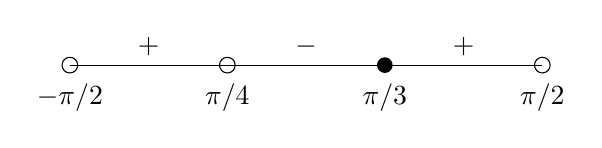
\begin{tikzpicture}	
			\draw
			(0,0) node[circle,draw,inner sep=2pt,label=below:$-\pi/2$](a){}
		-- (2,0) node[circle,draw,inner sep=2pt,label=below:$\pi/4$](b){} node[midway,above]{$+$}
		-- (4,0) node[circle,fill,inner sep=2pt,label=below:$\pi/3$](c){}node[midway,above]{$-$}
		-- (6,0) node[circle,draw,inner sep=2pt,label=below:$\pi/2$](d){} node[midway,above]{$+$};
		\end{tikzpicture} \\
		&x\in\interval[scaled,open left]{\frac{\pi}{4}}{\frac{\pi}{3}}
		\intertext{Domain of inverse is range of function}
		&\boxed{\text{Range: }\interval[scaled,open left]
			{\frac{\pi}{4}}{\frac{\pi}{3}}} \\
	\end{align*}
	\end{multicols}
\end{itemize}

\section*{Problem 5}
\begin{itemize}
\item[(a)]
	\begin{align*}
		y&=\tan\left(\frac{x}{2}\right)+\cot\left(\frac{x}{2}\right)
	\end{align*}
	Period of $\tan x$, $\cot x$ are $\pi$. There is a horizontal
	dilation by a factor of 2, making their respective periods
	$2\pi$. The LCM of $2\pi$ and $2\pi$ is $2\pi$, so the period of
	$y$ is \boxed{2\pi}.
	
\item[(b)]
\begin{align*}
	y&=\frac{\tan\frac{x}{3}+\tan\frac{2x}{3}}
		{1-\tan\frac{x}{3}\tan\frac{2x}{3}} \\
	&=\tan\left(\frac{x}{3}+\frac{2x}{3}\right) \\
	&=\tan x
	\intertext{\centering{\boxed{\text{Period: }\pi}}} \\
\end{align*}

\item[(c)]
\begin{align*}
	f\left(x\right)&=\cos2x+3\sin\left(3x-\frac{\pi}{3}\right)-
		\frac{1}{2}\cot\left(\frac{4x}{5}+1\right)+7
\end{align*}
\begin{multicols}{3}
$\begin{aligned}
	&\text{Period }\cos2x \\
	=&\frac{1}{2}\cdot2\pi \\
	=&\pi \\
\end{aligned}$
\vfill\null\columnbreak
$\begin{aligned}
	&\text{Period }3\sin\left(3x-\frac{\pi}{3}\right) \\
	=&\frac{1}{3}\cdot2\pi \\
	=&\frac{2\pi}{3} \\
\end{aligned}$
\vfill\null\columnbreak
$\begin{aligned}
	&\text{Period }\frac{1}{2}\cot\left(\frac{4x}{5}+1\right) \\
	=&\frac{5}{4}\cdot\pi \\
	=&\frac{5\pi}{4} \\
\end{aligned}$
\end{multicols}

\begin{gather*}
	\text{LCM of $\pi$, $\frac{2\pi}{3}$, $\frac{5\pi}{4}$}=10\pi \\
	\therefore\boxed{\text{Period: }10\pi}
\end{gather*}

\end{itemize}

\pagebreak
\section*{Problem 6}
\begin{proof}
	\begin{vwcol}[widths={0.4,0.6},
		sep=.8cm, justify=flush,rule=0pt,indent=1em]

	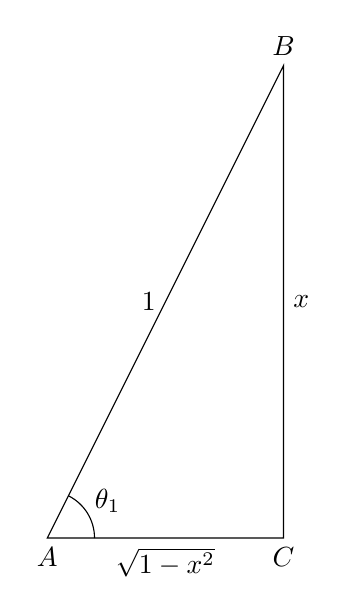
\begin{tikzpicture}[
		baseline=(current bounding box.north),
		ang/.style={draw, angle eccentricity=1.5,angle radius=0.6cm}
	]	
		\draw 
		(0,0) coordinate[label=below:{$A$}](A)
	 -- (3,0) coordinate[label=below:{$C$}](C) node[midway,below]{$\sqrt{1-x^2}$}
	 -- (3,6) coordinate[label=above:{$B$}](B) node[midway,right]{$x$}
	 -- cycle node[midway,above,left]{$1$}
	 	pic["$\theta_1$",ang]{angle=C--A--B};
	\end{tikzpicture}
	$\begin{aligned}[t]
		\\
		\text{Let }\theta&=\arcsin x \\
		\sin\theta&=\sin\left(\arcsin x\right) \\
		\frac{\text{opp}}{\text{hyp}}&=x \\
		\frac{BC}{AB}&=x \\
		\text{Let }BC&=x,\,AB=1 \\
		AC&=\sqrt{1-x^2} \\
		\\
		\tan\theta&=\frac{x}{\sqrt{1-x^2}}
	\end{aligned}$
	\pagebreak
	$\begin{aligned}[t]
		\\
		\tan\theta&=\frac{x}{\sqrt{1-x^2}} \\
		\tan\left(\arcsin x\right)&=\frac{x}{\sqrt{1-x^2}} \\
		\alignedintertext{Becuase the domain of $\arctan x$
			is $\mathbb{R}$, we can safely take the arctangent of both
			sides.}
		\arctan\left(\tan\left(\arcsin x\right)\right)
		&=\arctan\frac{x}{\sqrt{1-x^2}} \\
		\arcsin x&=\arctan\frac{x}{\sqrt{1-x^2}} \\
	\end{aligned}$
	\end{vwcol} 
\end{proof}

\end{document}
